\documentclass{scrartcl}
\usepackage[mathletters]{ucs}
\usepackage[utf8x]{inputenc}
\usepackage{amssymb}
\usepackage{amsmath}
\usepackage[usenames]{color}
\usepackage{hyperref}
\usepackage{wasysym}
\usepackage{graphicx}
\usepackage[normalem]{ulem}
\usepackage{enumerate}

\usepackage{listings}

\lstset{ %
basicstyle=\footnotesize,       % the size of the fonts that are used for the code
showspaces=false,               % show spaces adding particular underscores
showstringspaces=false,         % underline spaces within strings
showtabs=false,                 % show tabs within strings adding particular underscores
frame=single,                   % adds a frame around the code
tabsize=2,                      % sets default tabsize to 2 spaces
breaklines=true,                % sets automatic line breaking
breakatwhitespace=false,        % sets if automatic breaks should only happen at whitespace
}


\title{Desk Lamp Test}
\date{dinsdag 08 december 2020}
\author{}

\begin{document}

\maketitle

		\section{Desk Lamp Test}

Created Wednesday 28 October 2020



First test using following setup:



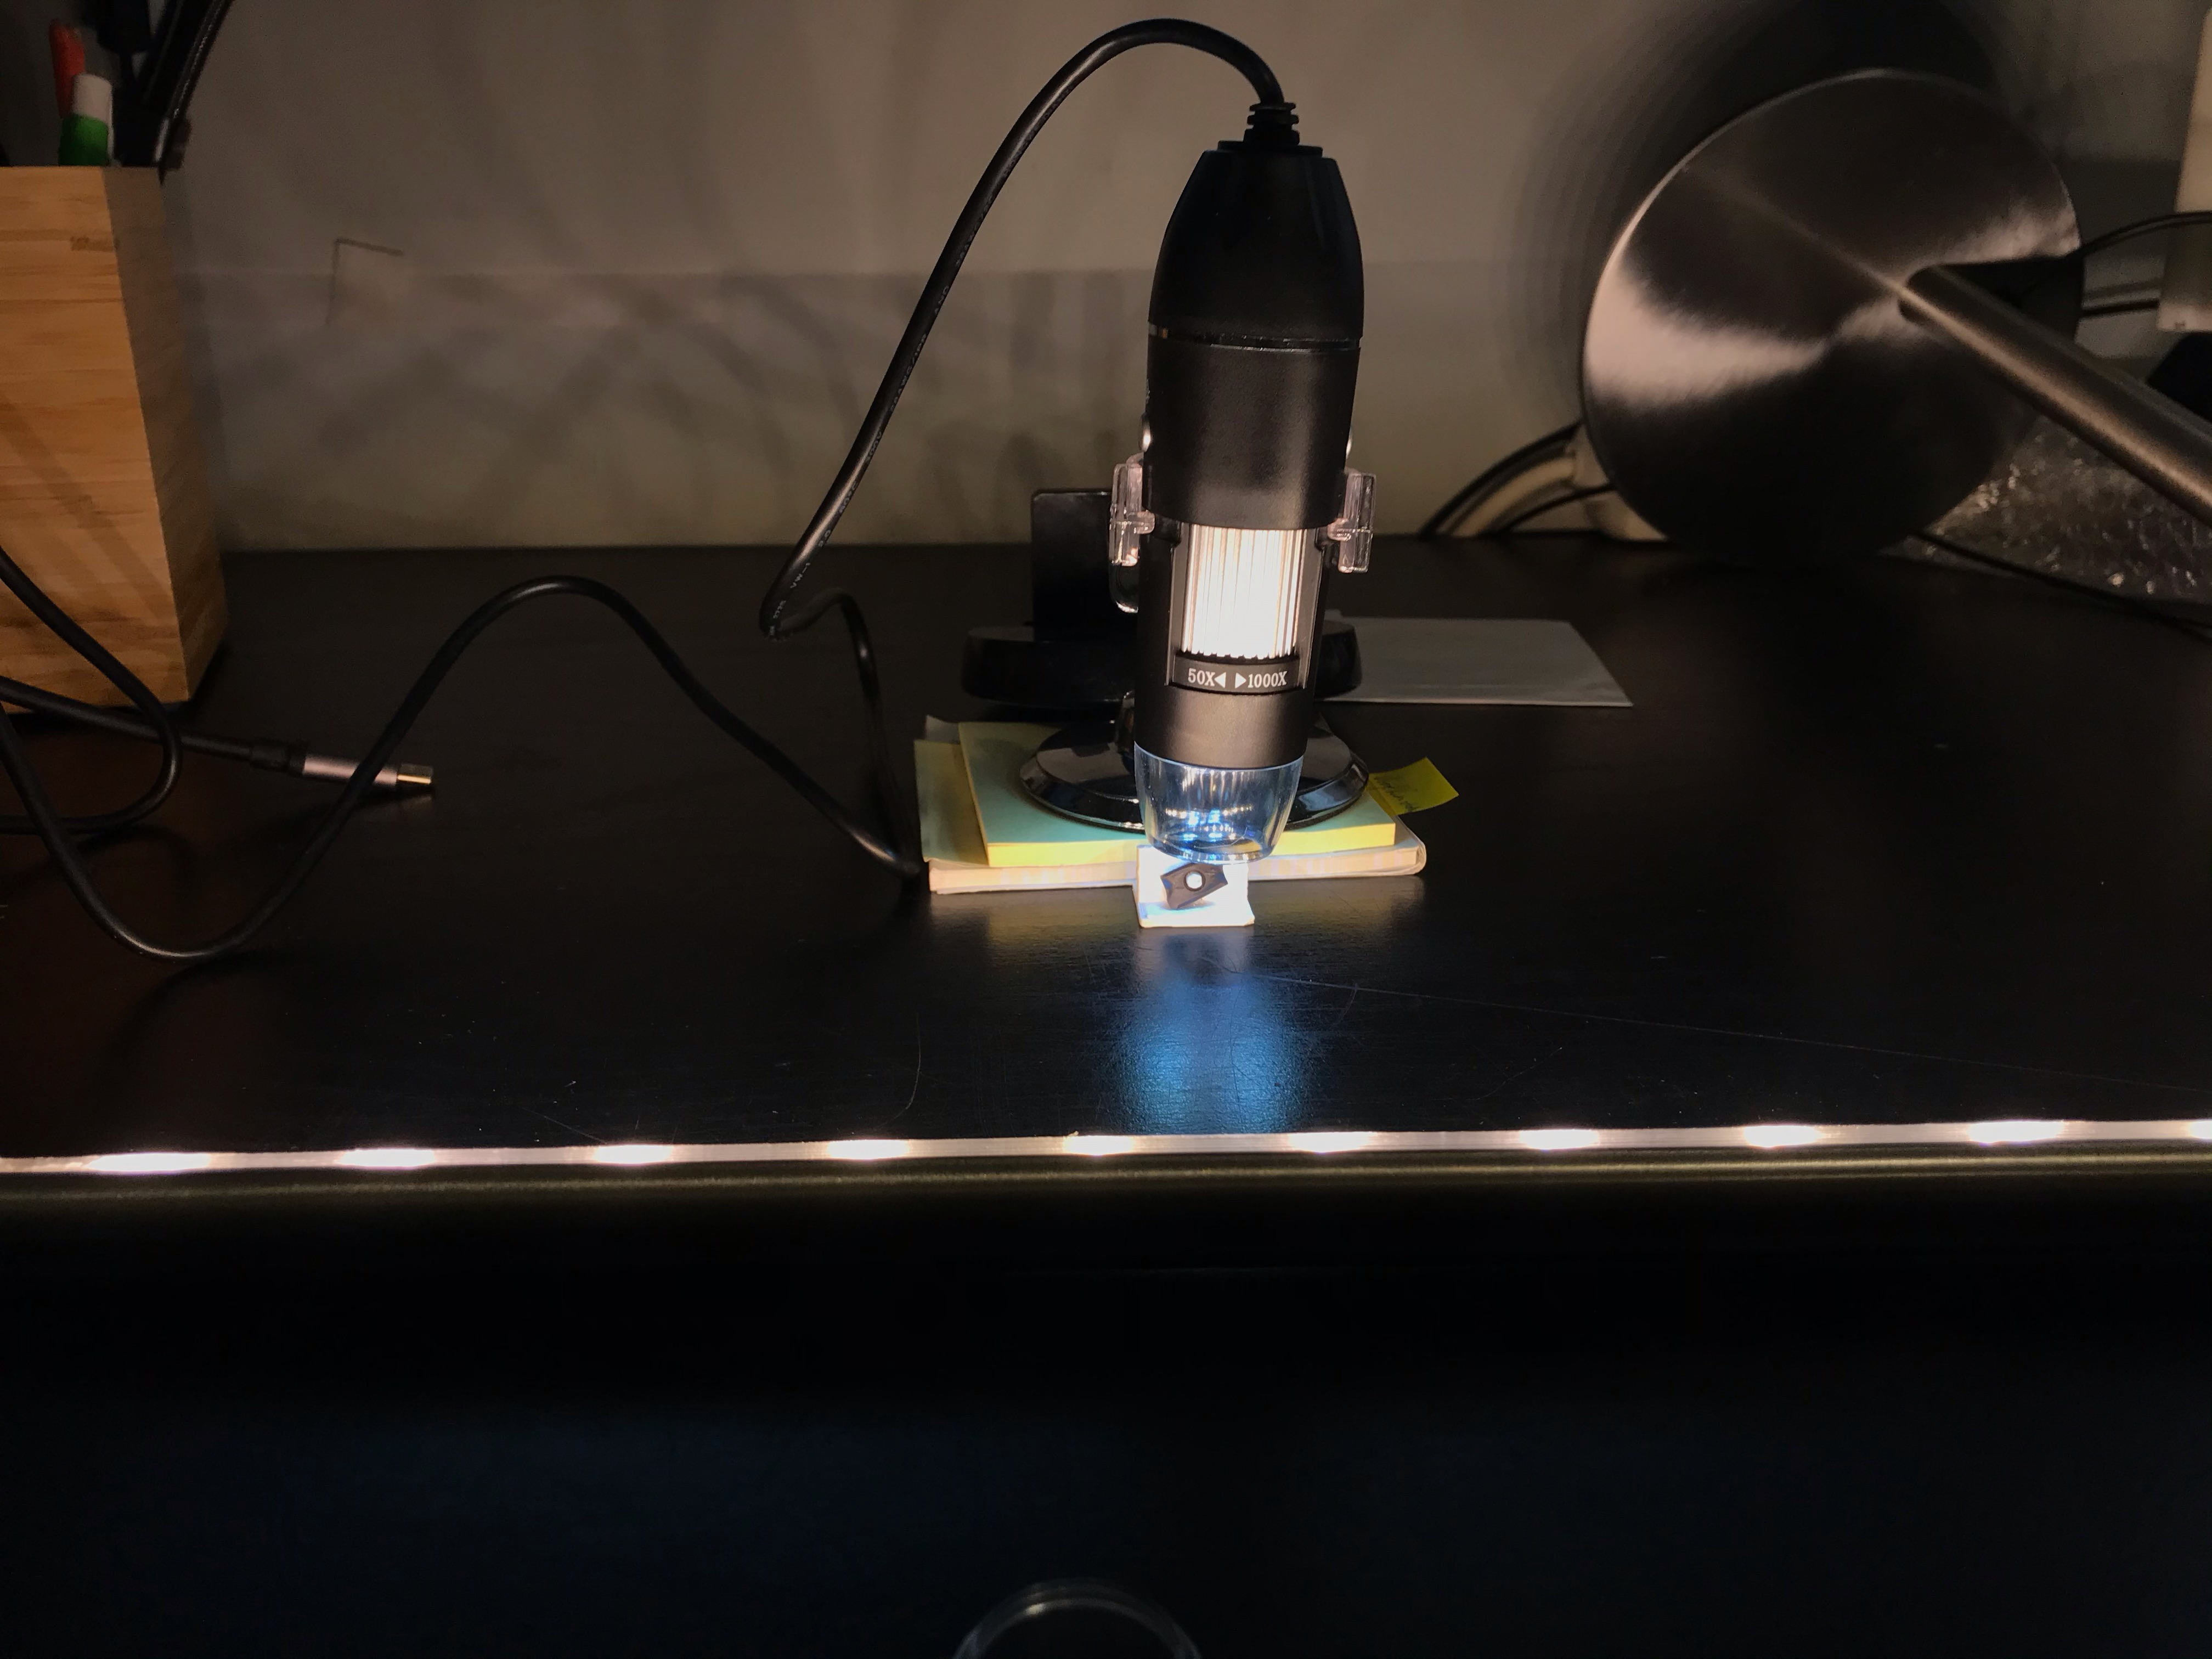
\includegraphics[width=4.166667in, keepaspectratio=true]{./Desk_Lamp_Test/eerste_setup_andere_richting.jpeg}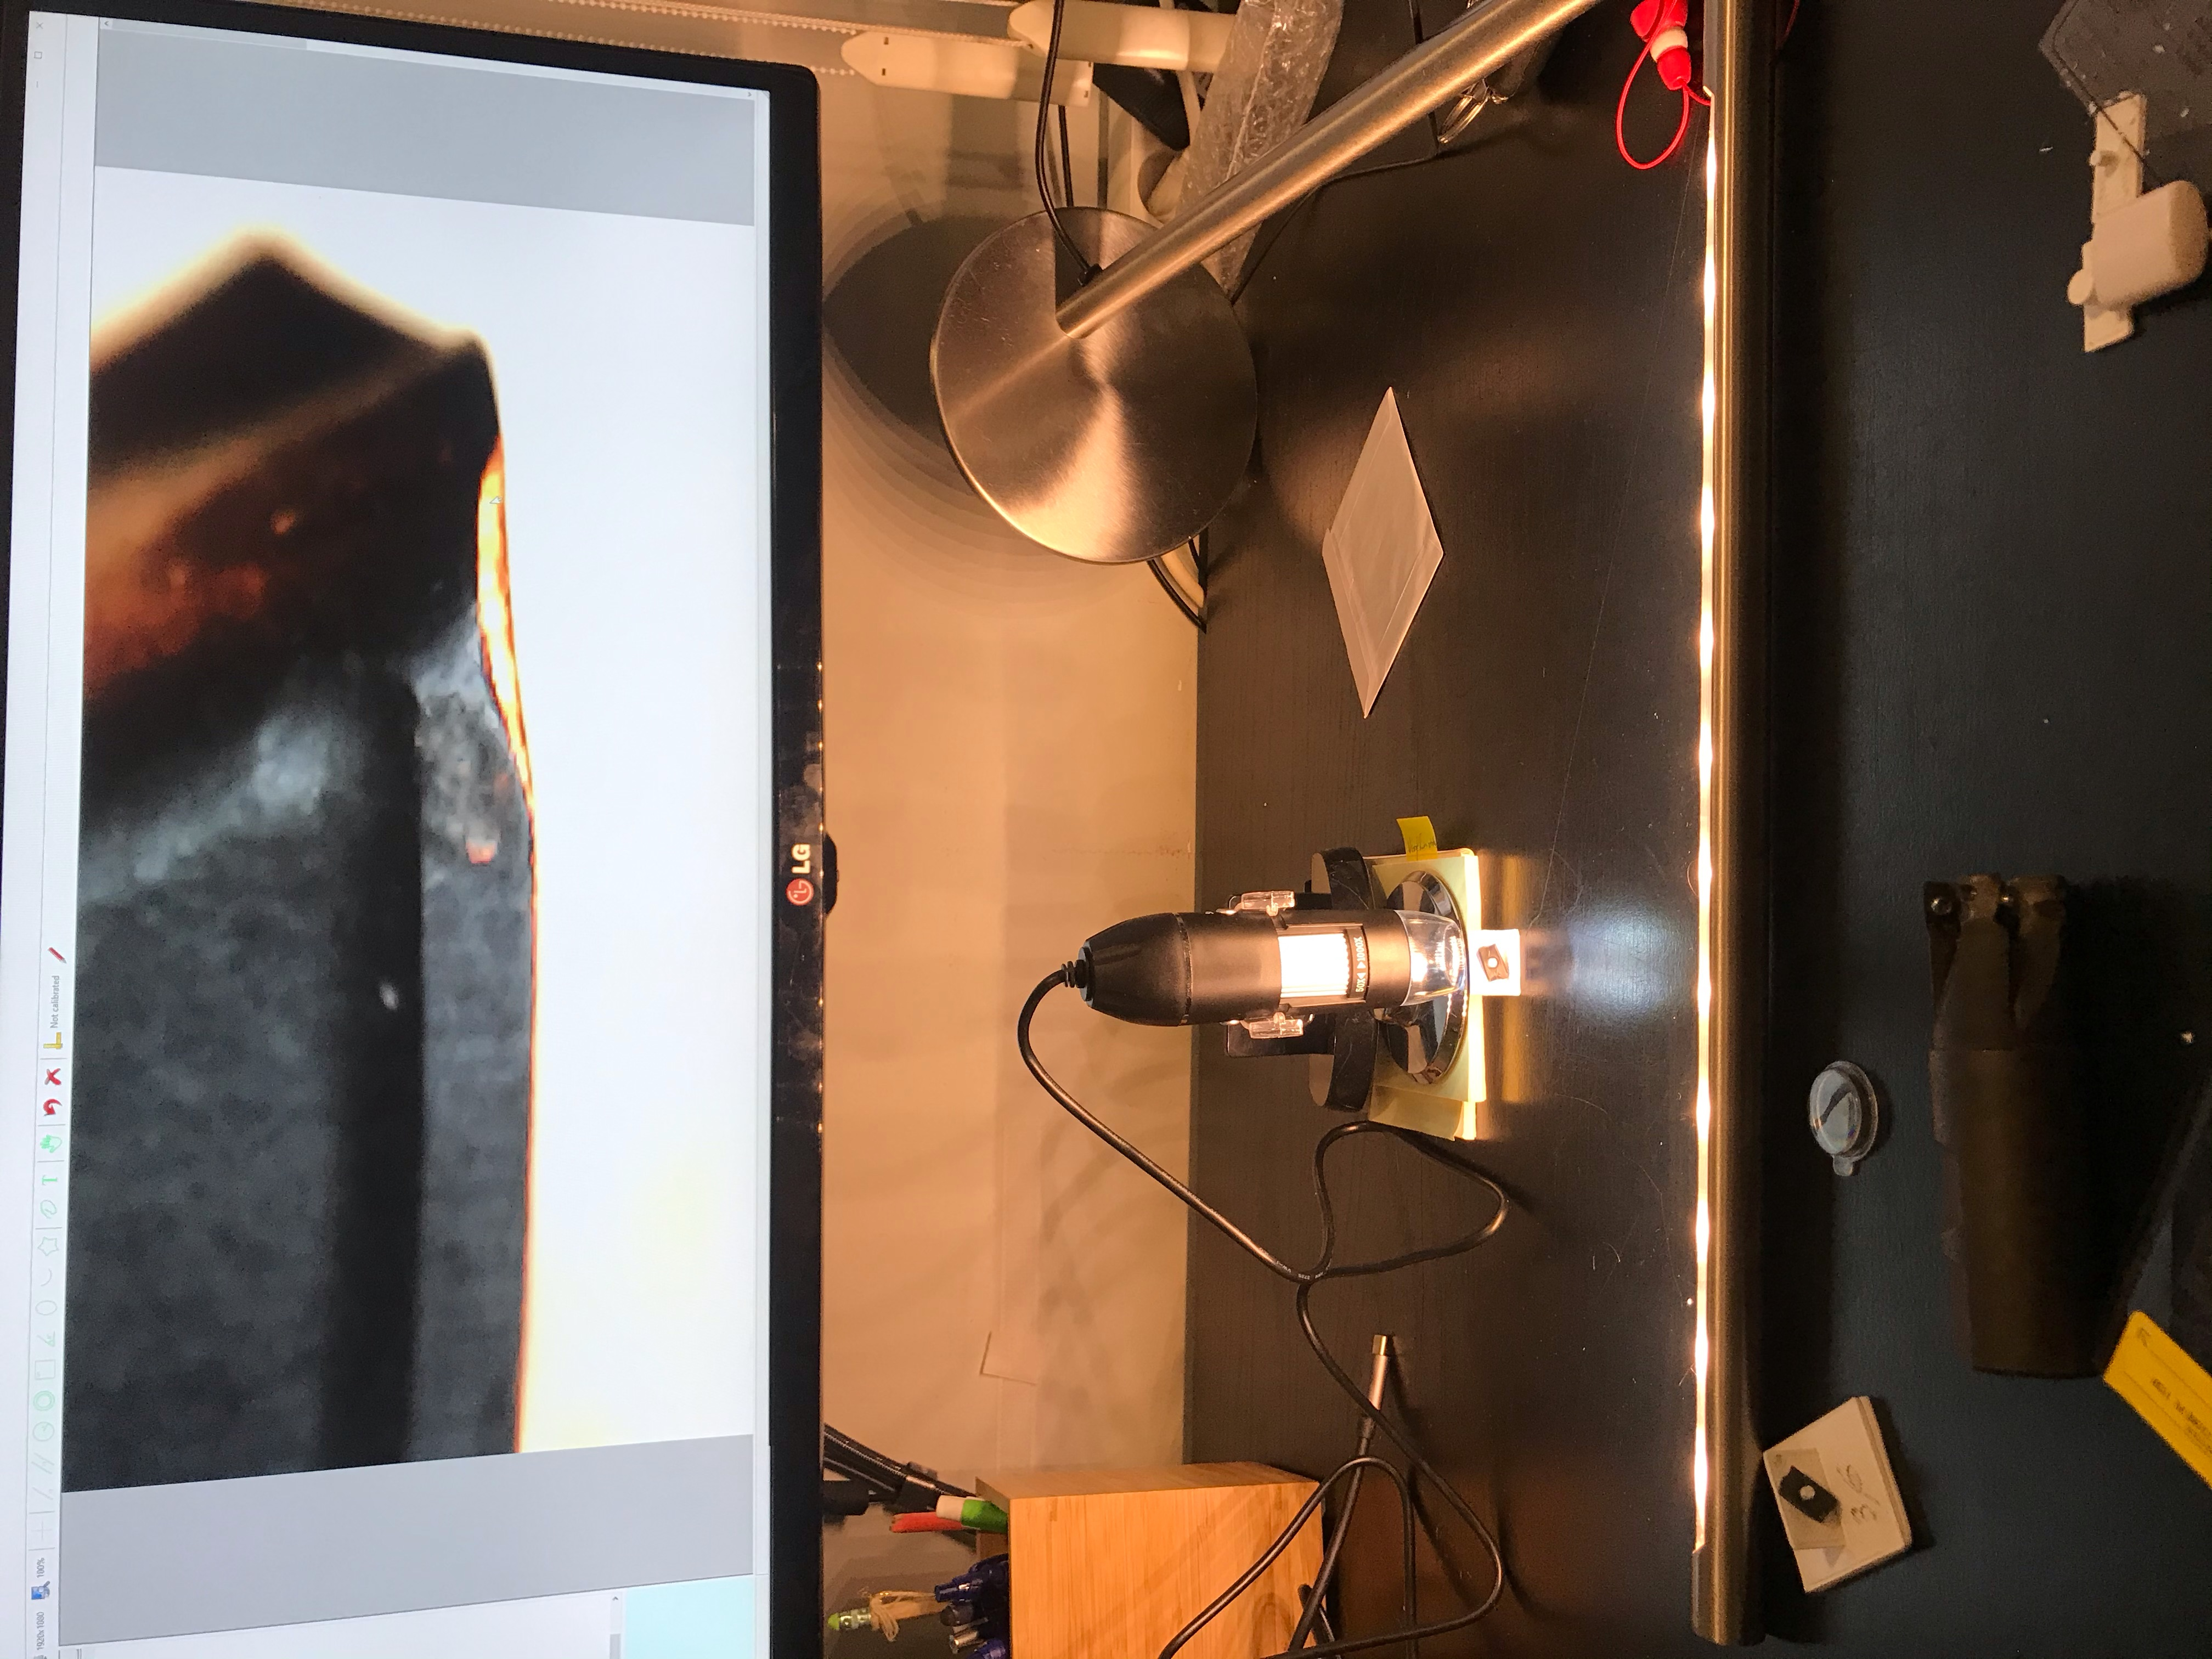
\includegraphics[width=4.166667in, keepaspectratio=true]{./Desk_Lamp_Test/eerste_setup_andere_richting_beeld2.jpeg}



This setup was using the top light of the camera. This light was good to be able to adjust the camera. Without the light, the errornous places where more visible. But the desk lamp had to much brightness. Therefor and to test other lighting conditions a led strip will be used for further tests. 



The result with this setup can be seen in the above picture on the screen. here can be seen that there is a bright white background behind the tool. In a new setup there will be tried to make the background as dark as possible to make sure only the bad part of the tool is clearly lighted.



The result of this is shown in the following picture where the light is blocked off of the rest of the tool and only the errornous part is lightened. This would be a good start to start creating a dataset.



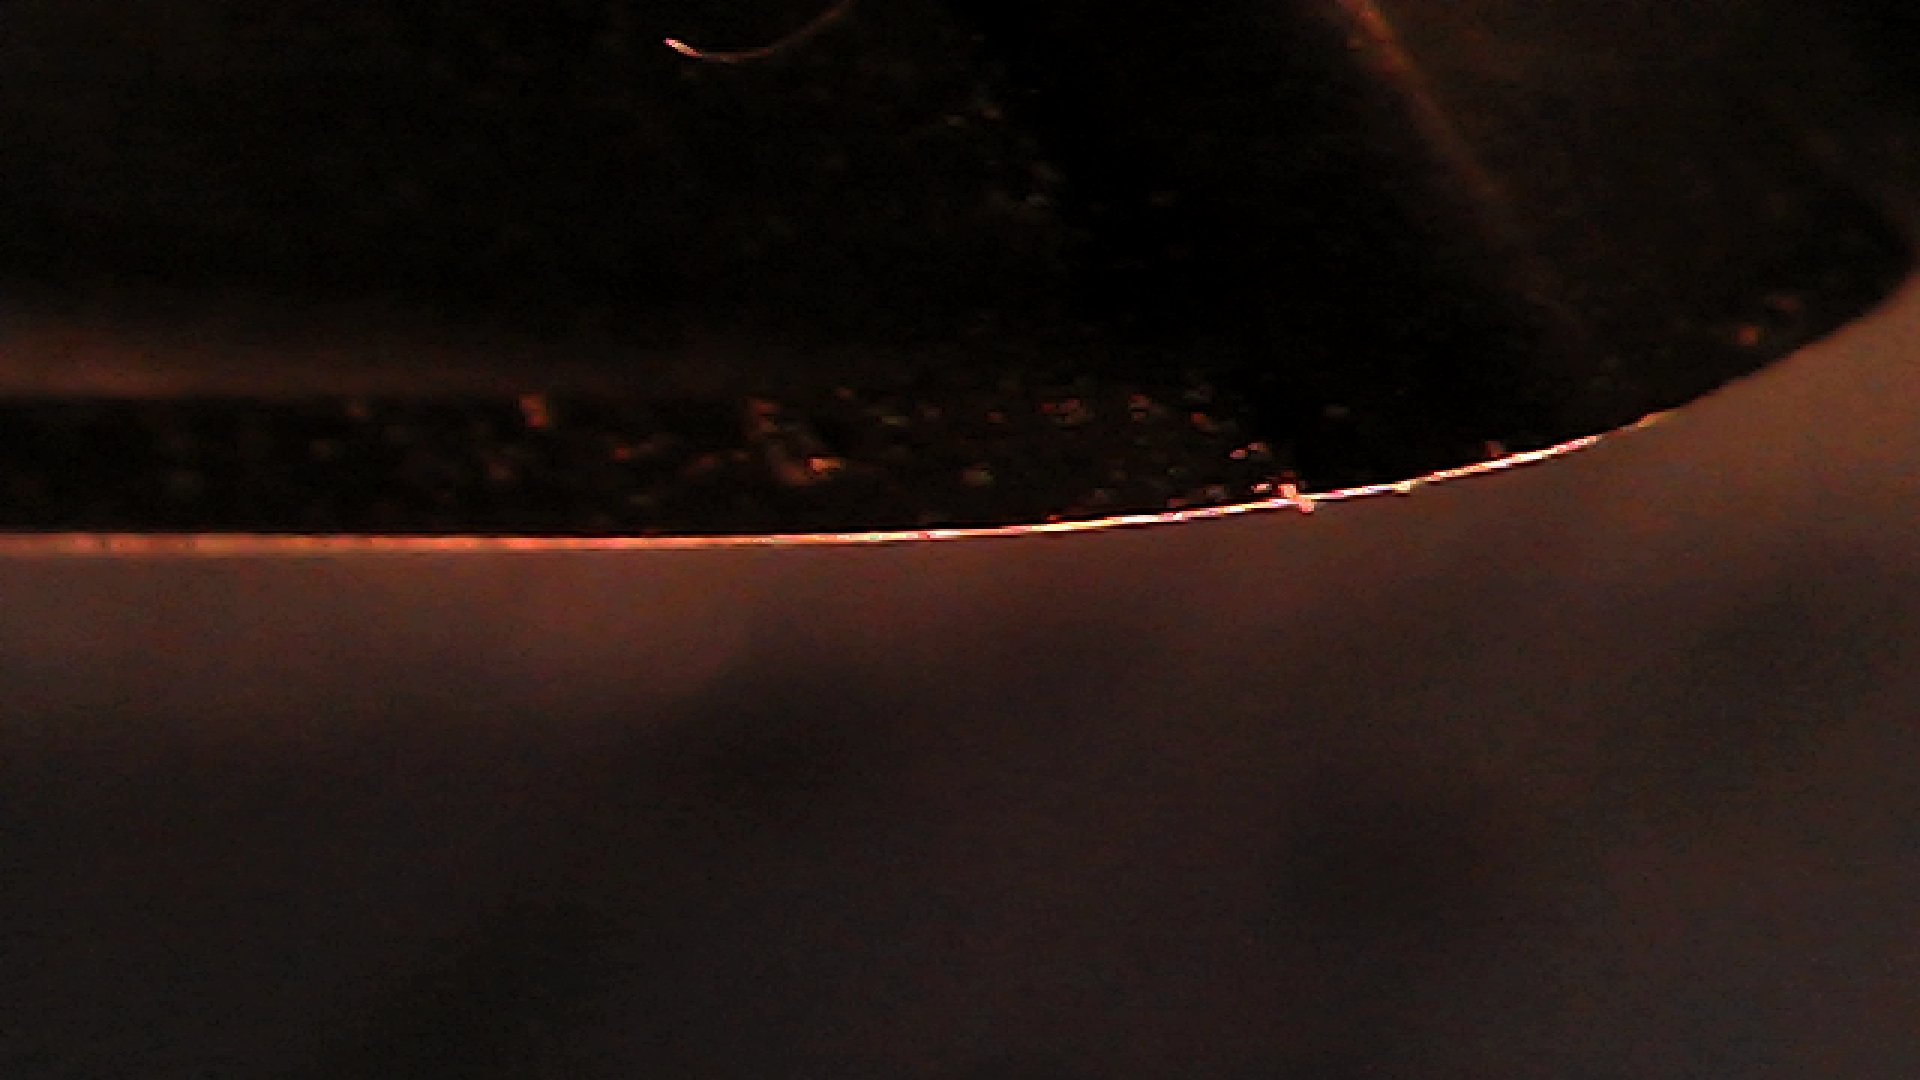
\includegraphics[width=4.166667in, keepaspectratio=true]{./Desk_Lamp_Test/eerste-opstelling_donkere_achtergrond2.jpg}



The color of the desk light set a good gradient of bad vs good sets. White areas are worn very hard while orange is not worn that hard.



By tilting the lamp up and down in a horizontal way, all the areas where ligthtend. 



The setup used for this lighting scene is described 



\end{document}
